% !TeX program = lualatex

\documentclass[12pt]{report}
\usepackage[table,xcdraw]{xcolor}
\usepackage[Glenn]{fncychap}
\usepackage[T1]{fontenc}
\usepackage[francais]{babel}
\usepackage{fontspec}
\usepackage{wrapfig}
\usepackage{graphicx}
\usepackage{soul}
\usepackage[colorlinks=true, linkcolor=black, urlcolor=black, citecolor=black]{hyperref}
% \usepackage[hyphens, spaces, obeyspaces]{url}
\usepackage[a4paper, width=175mm, top=25mm, bottom=25mm]{geometry}
\usepackage{parskip}
\usepackage{enumitem}
\usepackage{titlesec}
\usepackage{listings}
\usepackage{float}
\usepackage[final]{pdfpages}
\usepackage{tocbibind}
\usepackage{tocloft}
\usepackage{xpatch}
\usepackage{amsmath}
\usepackage{amsthm}
\usepackage{amsfonts}
\usepackage{graphics}
\usepackage{color}
% \usepackage[grey,utopia]{quotchap}
\usepackage{moreverb}
\usepackage{framed}
\usepackage{arabluatex}
%\usepackage[algo2e, french, onelanguage, ruled]{algorithm2e}
\setlist[itemize]{label=\textbullet}
\usepackage{fancybox, graphicx}
\usepackage{fancyhdr}
\pagestyle{fancy}   
\fancyhead{}
\fancyhead[C]{\leftmark}
\renewcommand{\headrulewidth}{0.4pt}
\renewcommand{\footrulewidth}{0.4pt}
\definecolor{light-gray}{gray}{0.90}
\usepackage{multirow}
\usepackage{soul}
\usepackage{graphicx}
\usepackage[utf8x]{inputenc}
\setcounter{secnumdepth}{3} 
\usepackage{dirtytalk}
\usepackage{csquotes}
\usepackage{mathtools}
\usepackage{amsmath}
\usepackage{tikz}
\usepackage{tikz-3dplot}
\usetikzlibrary{shapes,arrows,angles}
\usepackage[ruled,french,onelanguage]{algorithm2e}
\usepackage{multirow}
\usepackage[noend]{algpseudocode}
\usepackage{tabularx}  % for tabularx
% to make cells in  have decent spacing
\usepackage{diagbox}
\usetikzlibrary{arrows, positioning, automata}
\usepackage{array}
\usepackage{venndiagram}

\DeclareMathOperator*{\argmax}{arg\,max}

\newsavebox{\picbox}
\newcommand{\cutpic}[3]{
	\savebox{\picbox}{\includegraphics[width=#2]{#3}}
	\tikz\node [draw, rounded corners=#1, line width=4pt,
	color=white, minimum width=\wd\picbox,
	minimum height=\ht\picbox, path picture={
		\node at (path picture bounding box.center) {
			\usebox{\picbox}};
	}] {};}


\begin{document}
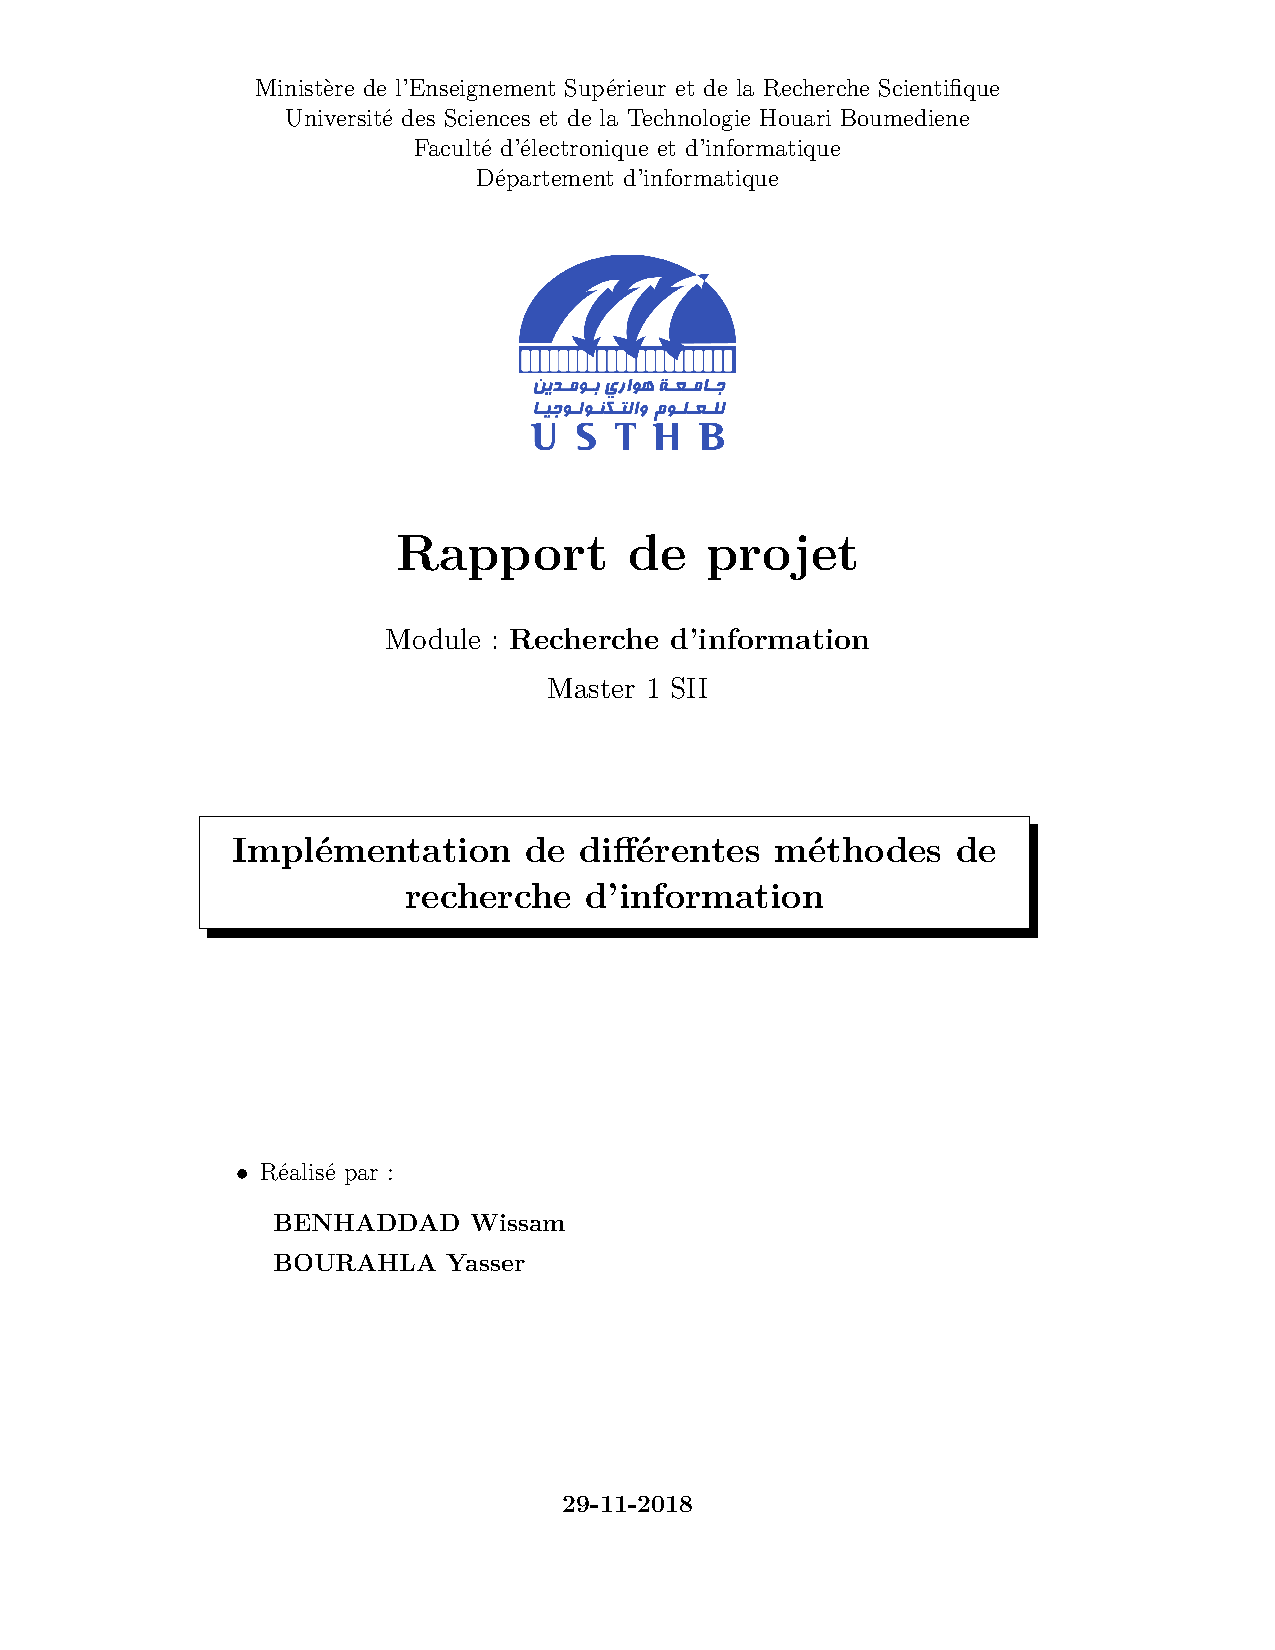
\includepdf[pages=1]{Page_garde.pdf} 
\tableofcontents
\listoffigures
\listoftables


\pagenumbering{arabic}
\newpage
%\title{Réalisation d'un assistant virtuel intelligent pour ordinateurs}
%\author{W.Benhaddad, Y.Bourahla}

\setlist[itemize]{label=\textbullet}

	\tikzstyle{decision} = [diamond, draw, fill=blue!20, 
text width=4.5em, text badly centered, node distance=3cm, inner sep=0pt]
\tikzstyle{block} = [rectangle, draw,fill=blue!20, 
text width=10em, text centered, rounded corners, minimum height=7em]
\tikzstyle{line} = [draw, -latex']
\tikzstyle{cloud} = [draw, ellipse,fill=red!20, node distance=3cm,
minimum height=2em]



\chapter{Introduction}
	\section{Problématique et objectifs}
	\paragraph{}
	Au fil des années, et depuis l'explosion du volume de données dans disponible 
	sur Internet, il était devenu de plus en plus difficile aux utilisateur d'accéder 
	rapidement et efficacement aux sources d'informations, cette augmentation du niveau
	de complexité d'accès aux données a motivé les chercheurs a développer de nouvelles
	méthodes pour faciliter la recherche d'information.  
	\par
	Généralement, le processus recherche d’information peut être divisé en trois étapes
	comme le montre le schéma suivant : 
	
	\begin{center}
			\begin{tikzpicture}[node distance = 5cm, auto]
		% Place nodes
		\node [block] (step1) {représentation de la collection des documents (corpus)};
		\node [block, right of=step1] (step2) {l’interrogation initiée par l’utilisateur (compréhension et traitement des requêtes)};
		\node [block, right of=step2] (step3) {la récupération des documents pertinents.};
		% Draw edges
		\path [line] (step1) -- (step2);
		\path [line] (step2) -- (step3);
		
		\end{tikzpicture}
	\end{center}
	\par 
	L'une des applications les plus courantes et les plus connues de la recherche
	d'information est peut-être la récupération de documents textuels sur Internet. Avec sa
	croissance récente, Internet devient rapidement le principal média de communication
	pour les entreprises et l'information académique. Il est donc essentiel de pouvoir
	exploiter le bon document à partir de ce vaste océan d'informations. C'est en fait l'une
	des principales forces motrices pour le développement de la recherche documentaire. À
	ce jour, de nombreux systèmes relativement efficaces ont été développés.
	
	\par
	L'une des premières remarques qui viennent à l'esprit est : "comment rendre ce processus
 	aussi rapide et intuitif que possible, sans se soucier du volume de données dans le quel
 	l'information est recherchée ?", le but de ce projet est donc d'étudier les méthode 
 	proposées pour remédier à ce problème, de les implémenter sur machine, et de comparer 
 	leurs résultats et performance sur une corpus de test préalablement construit, tout cela 
 	dans l'optique de mieux comprendre pourquoi cette tâche(la RI) est si complexe et ardue.
	
	\section{Définitions}
	\paragraph{}
	Pour mieux comprendre le contexte dans le quel nous nous trouvons, nous allons définir
	quelques notions en rapport avec la \textbf{RI}:
		\subsection{La recherche d'information}
		\paragraph{}
		La RI\footnote{Recherche d'Information} peut être définie comme suit : 
		\begin{quote}
			\say{La signification du terme « Recherche d’information » peut être très large. Cependant,
				en tant que domaine d’étude académique il peut être défini comme le domaine qui étudie
				les méthodes permettant de trouver des informations pertinentes dans un corpus,
				composé d’une collection de documents non-structurés. Il s’agit essentiellement de
				faciliter d’accès de l’utilisateur à un grand volume de données}
		\end{quote}
		
		
		\subsection{L'indexation de documents}
		\paragraph{}
		L’indexation de documents est un l'opération qui consiste à organiser un ensemble de documents 
		et faciliter ultérieurement la recherche de contenu dans cette collection. Pour y arriver le 
		système essaye de construire un index(une liste de descripteurs à chacun desquels est associée 
		une liste des documents et/ou parties de documents auxquels ce descripteur renvoie), dans ce
		projet nous allons utiliser deux méthodes d'indexations : 
		\subsection{Indexation par fichier inverse}
		\paragraph{}
		Ce modèle d'indexation construit une représentation de correspondance entre un document 
		\textbf{d} et une entité (généralement un terme) \textbf{t} contenu dans le document,
		construisant ainsi un dictionnaire \textbf{Dico} dont les entrés sont de la forme suivante :
		\begin{equation*}
			Dico[d,t] \rightarrow V
		\end{equation*} 
		où $V$ peut être une mesure 
		qualifiant l'appartenance du terme \textbf{t} dans le document \textbf{d} (fréquence
		d'apparition, poids, position ... ).dans ce projet nous utiliserons 
		
		\subsection{La mesure TF : }
		\textbf{TF} pour \textbf{Term-Frequency} est une mesure qui donne simplement combien un terme
		est important dans un document \textbf{d}, sa formule la plus simple est la suivante  : 
		\begin{equation*}
			TF[w,d] = nombre\_occurence\_w\_dans\_d
		\end{equation*}
		La forme normalisé est la suivante : 
		
		\begin{equation*}
		TF[w,d] = \frac{nombre\_occurence\_w\_dans\_d}{nombre\_total\_termes\_dans\_d}
		\end{equation*}
		
		\subsection{La mesure IDF}
		\textbf{IDF} pour \textbf{Inverse Document Frequency} est une mesure quant à elle qui nous
		renseigne sur combien de gain d'information un terme peut fournir par rapport à \textbf{tout}
		les documents, sa formule est la suivante : \par
		Soient : 
		\begin{itemize}
			\item $w$ le terme au quel on s'intéresse.
			\item $d_w$ le nombre de document où le terme $w$ apparaît (i.e $1 + |\lbrace d \in D , TF[w,d] \neq 0 \rbrace $|)
			\item $D$ l'ensemble de tout les documents.
		\end{itemize}
		\begin{equation*}
			IDF[w,D] = \log{\frac{|D|}{d_w}}
		\end{equation*}
		
		\subsection{TF-IDF comme poids d'un document}
		La mesure \textbf{TF-IDF} est le produit entre les deux mesures qui la composent, ainsi : 
		\begin{equation*}
			TF-IDF[w,d,D] = TF[w,d] * IDF[w,D]
		\end{equation*}
		\paragraph{Analyse} : cette mesure représente le poids d'un terme $w$ dans un document $d$ par rapport à un corpus
		(ensemble de documents) $D$, ce poids va donc indiquer à quel point un terme est présent dans un petit nombre de 
		documents, en effet TF-IDF donne la priorité (attribut un poids élevé) aux termes qui apparaissent le plus souvent
		dans le document visé, et qui sont peu fréquent dans tout le corpus en général, cela facilite donc le choix du(ou des)
		document(s) pertinent(s) à renvoyer.
		
		
		\subsection{Méthodes de recherche}
		\paragraph{}
		Maintenant que nous avons notre modèle d'indexation des documents de notre collection, nous devons ensuite définir
		les méthodes d'interrogation de cette dernière, plusieurs modèles ont vu le jour à travers le développement de la 
		RI, dans ce TP nous avons choisis de nous intéresser à 3 d'entre eux : 
			\subsubsection{Modèle booléen}
			\paragraph{}
			Le modèle booléen est un est tout premier modèle à avoir vu le jour, et est encore à ce jour très utilisé, son
			principe est simple, ayant :
			\begin{itemize} 
				\item une collection de documents $D$ tel que :
				\begin{equation*}
					D = \lbrace D_1,D_2,...,D_n\rbrace
				\end{equation*}
				
				\item une collection de termes $T$ tel que : 
				\begin{equation*}
				T = \lbrace T_1,T_2,...,T_m\rbrace
				\end{equation*}
				
				\item un index de terme/document $I$ tel que : 
				
				\[
				T[t_i,d_j]= 
				\begin{cases}
				1,& \text{si } t_j \in d_i\\
				0,              & \text{sinon}
				\end{cases}
				\]
				
				\item une requête en forme normale conjonctive : ( une conjonction de clauses )
				\begin{equation}
					Q = \lparen W_1 \lor W_2 \lor ... \rparen \land ... \land \lparen W_i \lor W_{i+1} ... \rparen
				\end{equation}
			\end{itemize}
			\par 
			Le but du modèle est, ayant reçu une requête $Q$, lo modèle va parcourir chaque termes dans une clause et 
			retourner l'ensemble $S_i$ des unions des sous ensembles $S_{i,j} $des documents qui contiennent le terme
			$W$ en question, ce processus est répété autant de fois qu'il y a de clauses dans $Q$. À la fin de ce parcours 
			un ensemble $S$ final sera construit à partir de l'intersection des ensembles $S_i$ construits auparavant.
			L'algorithme suivant résume ce traitement : 
			
			\begin{algorithm}[H]
				\caption{Évaluation modèle booléen}
				\SetKwInOut{Input}{Entrée}\SetKwInOut{Output}{Sortie}
				\SetKwFunction{cl}{Clauses}
				\SetKwFunction{contains}{Contient}
				
				\Input{($Q$ : requête en FNC , $I$ index terme/document , $D$  : l'ensemble des documents , $T$ l'ensemble des termes)}
				\Output{($S$ : Ensemble des documents pertinents)}
				
				
				\Begin
				{
					$S \gets \lbrace \rbrace $
					\ForEach{($c_i$ \in \cl{$Q$)}}
					{
						$S_i \gets \lbrace \rbrace$
						\ForEach{$t_j \in c_i$ }
						{
							$S_{i} \gets S_i \bigcup \lbrace d \in D , I[w,d] \neq 0 | w \in T \rbrace$
						}
					$S \gets S \bigcap S_i$
					}
					
				}
				\KwRet{$S$}
			\end{algorithm}
			
			
			\subsubsection{Modèle Vectoriel}
			\paragraph{}
			Le modèle vectoriel se veut plus détaillé que son prédécesseur, en effet l'idée est de
			modéliser chaque document $d_i$ de la collection $D$ comme étant un vecteur $v_{d_i}$,dans
			l'espace vectoriel $EV$ dont les vecteurs : 
			\[
			B = 
				\lbrace
					W_1 = (1,0,...,0) , W_2 = (0,1,...,0) , ... , W_n=(0,0,...,1)           \\[0.3em]
				\rbrace
			\]
			ont forment la \textbf{base}
			\par
			Autrement dit, considérant un document $d_i$ contenant les termes $\lbrack w_1 , w_2 , w_3 \rbrack$ 
			et l'ensemble des termes $T = \lbrace w_1 ... w_n \rbrace$, ce dit vecteur $d_i$ sera 
			représenté comme combinaison linéaire de $B$ (la base de $EV$) tel que : 
			\[
			\vec{d_i} =
				 \alpha_1*\vec{W_1} + \alpha_2*\vec{W_2} + ... + \alpha_n*\vec{W_n}
			\]
			\par Tel que :
			\[
			\alpha_i  =  
			\begin{cases}
				poids[w_i,d_i],	& \text{si } w_i \in d_i\\
				0,              & \text{sinon}
			\end{cases}
			\] 

			\paragraph{Exemple : }
			\begin{center}
				\tdplotsetmaincoords{60}{120}
				\begin{tikzpicture}[tdplot_main_coords]
				% Axes
				\draw [->] (0,0,0) -- (3,0,0) node [below left] {$w_1$};
				\draw [->] (0,0,0) -- (0,3,0) node [right] {$w_2$};
				\draw [->] (0,0,0) -- (0,0,3) node [above] {$w_3$};
				% Vectors
				\draw [->, thick] (0,0,0) -- (-2,2,3);
				\draw [->, thick] (0,0,0) -- (-2,0,1);
				% Ticks
				\foreach \i in {1,2}
				{
					\draw (-0.1,\i,0) -- ++ (0.2,0,0);
					\draw (\i,-0.1,0) -- ++ (0,0.2,0);
					\draw (-0.1,0,\i) -- ++ (0.2,0,0);
				}
				% Labels
				\node [below right] at (-2,2,3) {$d_1$};
				\node [above  left] at (-2,0,1) {$d_2$};
				\end{tikzpicture}
			\end{center}
			\paragraph{Évaluation d'un requête $Q$} 
			Tout comme un document $d$, une requête $q$ est une combinaison linéaire de $B$, la requête 
			est donc un vecteur dans l'espace vectoriel $EV$, le modèle procède au calcul d'une fonction
			de similarité $Sim$ entre le vecteur $\vec{q}$ et l'ensemble des vecteur
			$\lbrace \vec{d_1} , \vec{d_2}, ... , \vec{d_n}\rbrace$ et de sélectionner les \textbf{k} 
			vecteurs document qui maximisent $Sim$, plus formellement , ayant : 
			\begin{itemize}
				\item $D$ l'ensemble des vecteurs documents 
				\item $q$ le vecteur requête
				\item $r$ le vecteur réponse
			\end{itemize}
		
			\[
				\vec{r} = k\_argmax_{d_i} (Sim(\vec{q},\vec{d_i}))
			\]
			
			\paragraph{}
			Pour calculer la similarité entre deux vecteurs $\vec{v_1}$ et $\vec{v_2}$, nous avons testé quatre
			méthodes : 
			
			\paragraph{Produit interne :}
			Du point de vue théorique, le produit interne(qui est une généralisation du produit scalaire) donne
			une quantification du degré de similarité entre deux vecteurs(en terme de magnitude(force,intensité..)
			et de directions(opposés,quasi similaires ... ), ainsi cette mesure tend à favoriser deux vecteurs
			qui \textbf{pointent vers la même direction}. Cette vision est très abstraite, mais s'applique très 
			bien dans le cadre de la représentation par modèle vectoriel, en effet si nous disposons de deux
			vecteurs documents $\vec{d_1}$ et $\vec{d_2}$ comme représentés dans le plan orthonormé suivant: 
			
			\begin{figure}[H]
				\centering
				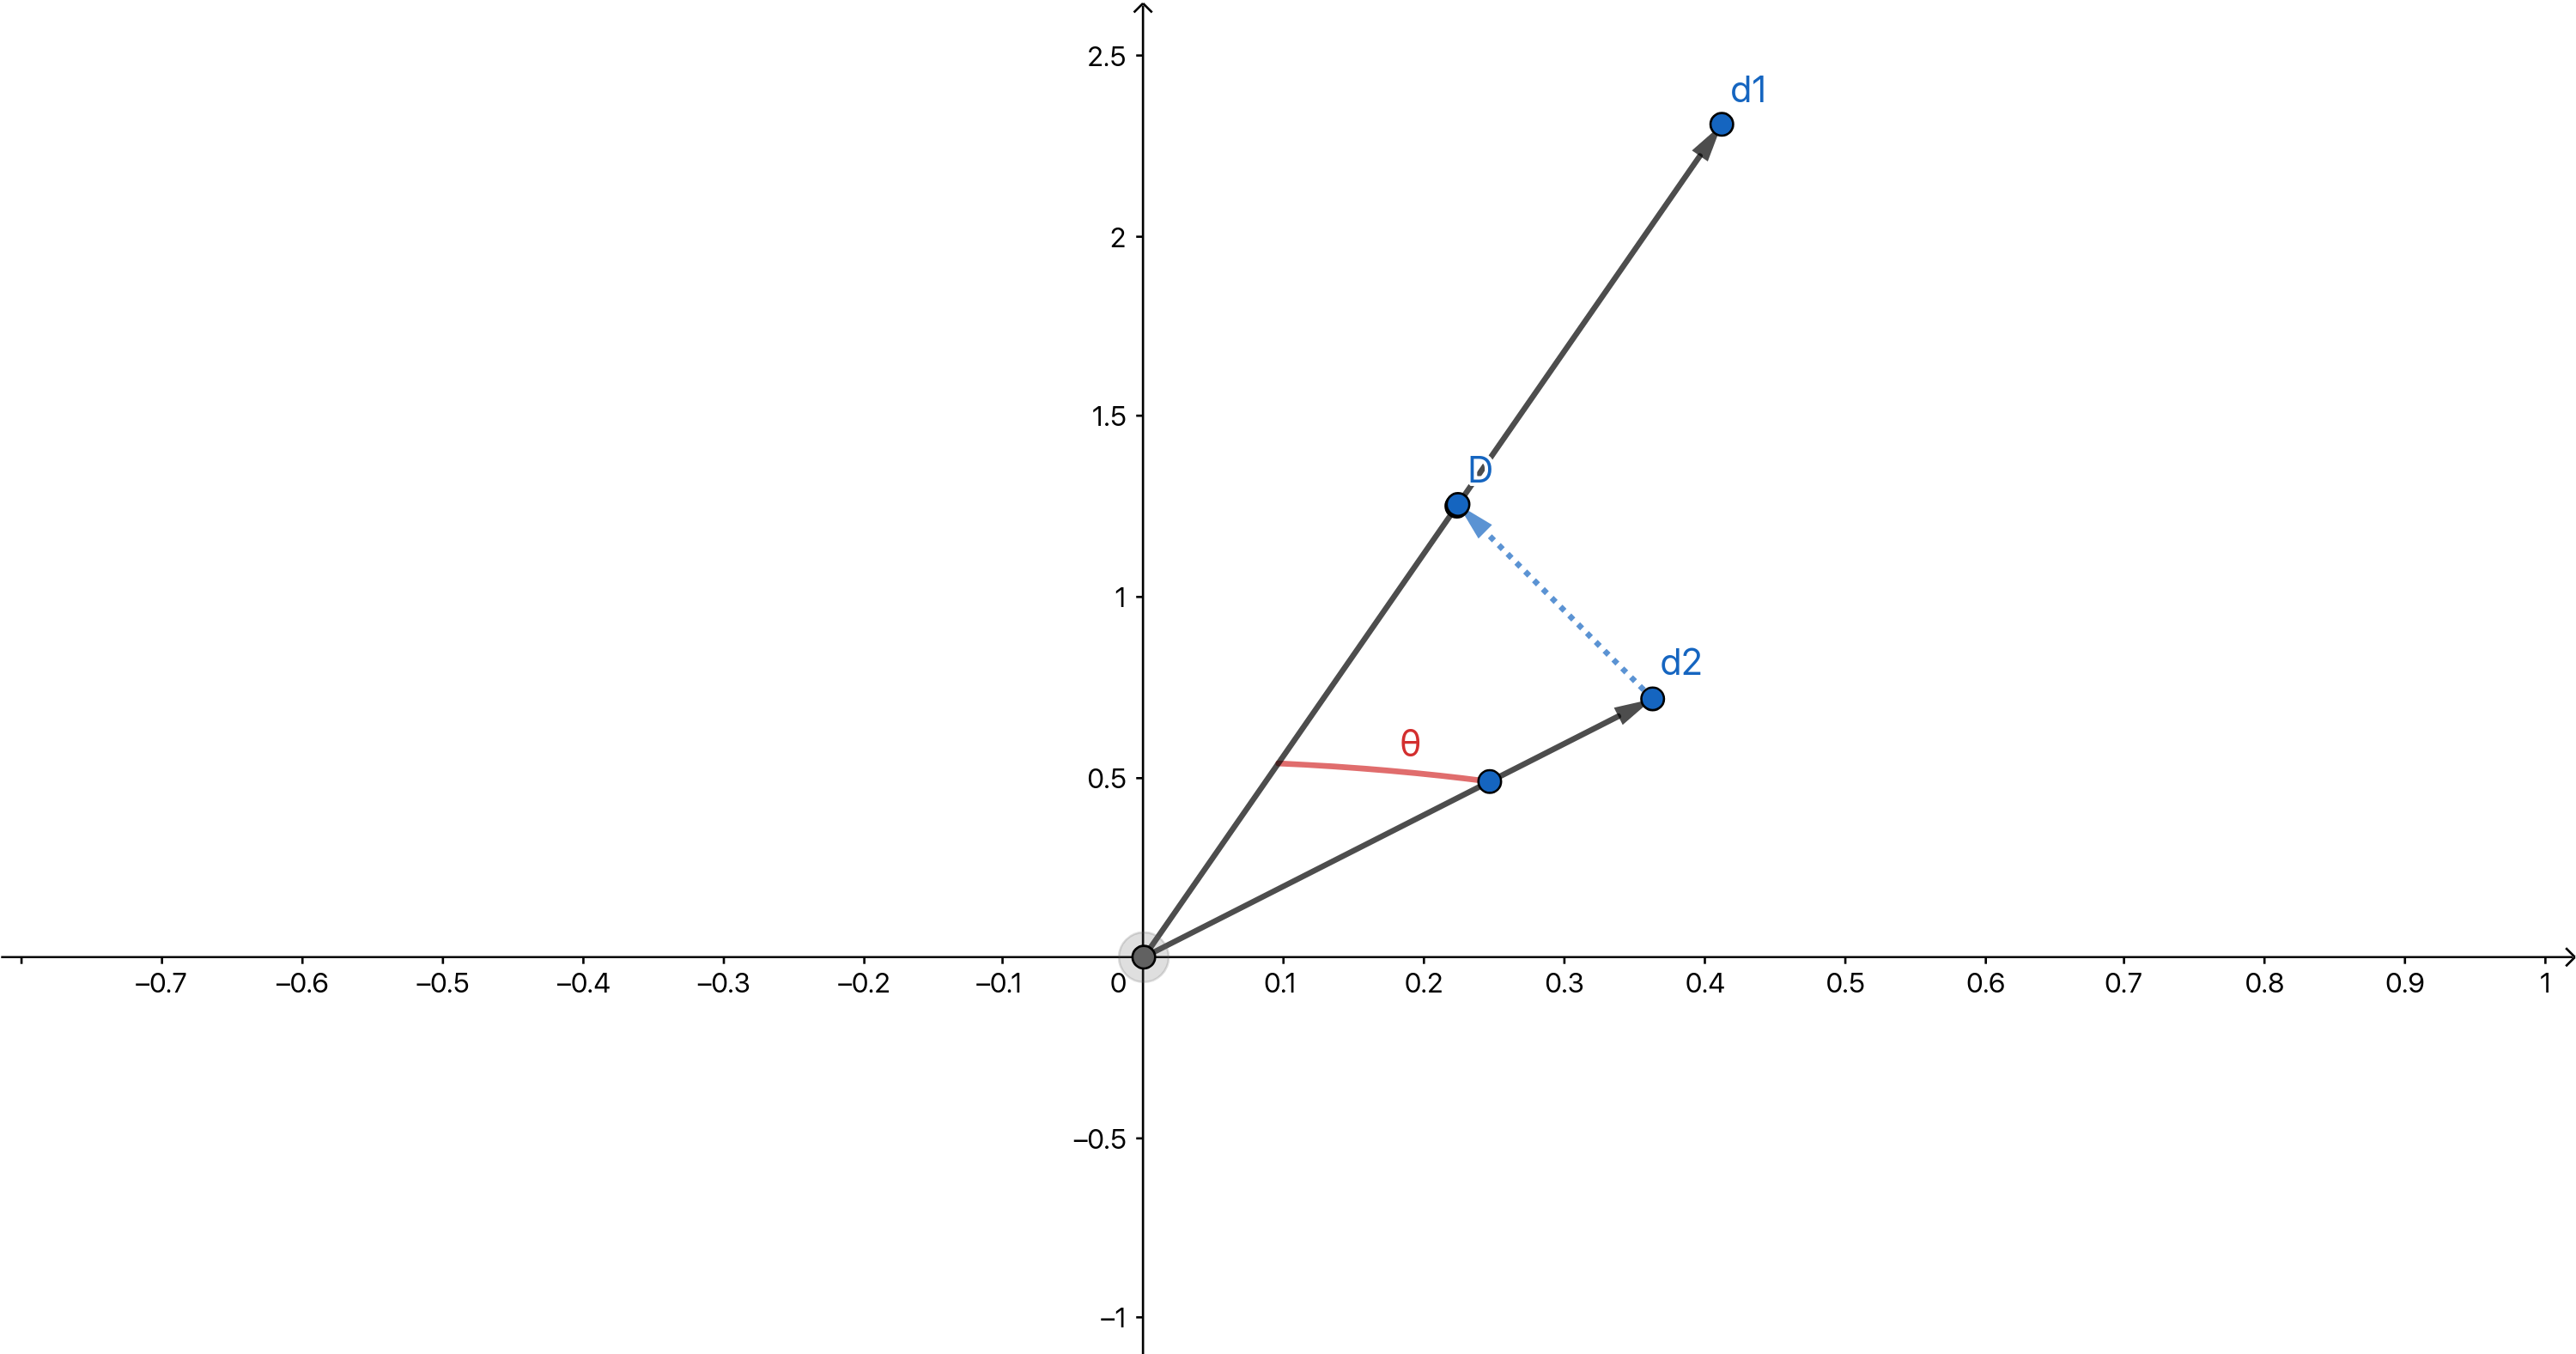
\includegraphics[width=0.75\linewidth]{images/geogebra-export.png}
			\end{figure}
			
			
			\par 
			Le produit scalaire grandit quand le nombre de composantes similaires augmente aussi, ainsi pour une
			requête $\vec{q} = \sum_{i=1}^{n} \alpha_i*w_i$ et un ensemble de documents
			$D = \lbrace\vec{d_i},...,\vec{d_n}\rbrace$, la similarité $Sim$ entre $q$ et un document $d_i$ est
			définie comme le produit scalaire : 
			\[
				Sim(q,d_i) = \vec{q} . \vec{d_i} = \sum_{j=1}^{n} q_j * d_{i,j}
			\]
			\par 
			Plus cette quantité est grande plus, un document $d_i$ est pertinent par rapport à la requête $q$.
			
			
			\paragraph{Similarité cosinus :}
			Très liée à la similarité par produit interne, cette mesure essaye de normaliser le degré de 
			similarité entre deux vecteurs(document avec document ou document requête), cela en calculant 
			le cosinus de l'angle entre ces deux vecteurs, par définition si deux vecteurs $\vec{v_1}$ 
			et $\vec{v_2}$ sont perpendiculaires, alors $ cos(\overrightarrow{v_1,v_2}) = 0$, ainsi deux documents
			seront non similaires si leurs vecteurs associés ne points pas vers la même direction, par 
			contraste, deux documents sont totalement similaires si l'un des leurs vecteurs représentant
			est un un scalaire de l'autre, c.à.d : $\vec{v_1} = \alpha * \vec{v_2}$, ainsi :
			$ cos(\overrightarrow{v_1,v_2}) = 1$, de ce fait la mesure de similarité est une quantité 
			qui prend ses valeurs dans l'intervalle $[0,1]$.\par 
			Pour implémenter son calcul, nous pouvons utiliser la formule du produit scalaire
			
			\begin{equation*}
				\begin{gathered}
				\vec{v_1}.\vec{v_2} = \parallel \vec{v_1}\parallel * \parallel \vec{v_2} \parallel  * cos(\overrightarrow{v_1,v_2}) \\\\
				cos(\overrightarrow{v_1,v_2}) = \frac{\sum_{i=1}^{n} v_{1,i} * v_{2,i} }
													{\sqrt{\sum_{i=1}^{n} v_{1,i}^2} * \sqrt{\sum_{i=1}^{n} v_{2,i}^2} }
				\end{gathered}
			\end{equation*}
			
			
			\paragraph{Coefficient de Jaccard : }
			Nous pouvons aussi tacler ce calcul de similarité d'un point de vue ensembliste, en utilisant 
			diverses mesures comme l'indice de \textbf{Jaccard}, cette mesure essaye de dénombrer les 
			éléments communs entre deux ensembles, en effet soit l'ensemble des documents des termes $T_i$
			apparaissant dans le document $d_i$, et $Q$ l'ensemble des termes apparaissant 
			dans la requête $q$(nous verrons comment cette interprétation peut être traduite en opération
			linéaire incluant des vecteurs), et soit le schéma suivant :
			\begin{center}
				\begin{venndiagram2sets}[labelA={$T_i$}, labelB={$Q$}]
					\fillACapB
				\end{venndiagram2sets}
			\end{center}
			\par 
			La zone grisée(l'intersection) représente l'information pertinente, soit les documents qui sont à 
			la fois dans $T_i$ et dans la requête, pour quantifier cette amas d'information, l'indexe de 
			\textbf{Jaccard} calcule le quotient 
			\[
				Sim(Q,T_i) = \frac{|T_i \bigcap Q|}{|T_i \bigcup Q|} = \frac{|T_i \bigcap Q|}{|T_i|+|Q|-|T_i \bigcap Q|}
			\]
			\newpage
			\par en terme de vecteurs, la cardinalité de l'intersection $|T_i \bigcap Q|$ est remplacée
			par le produit scalaire $\vec{d_i}.\vec{q}$ et la cardinalité d'un ensemble $|T_i|$(resp. $|Q|$) 
			par le carré de sa magnitude $|\vec{d_i}|^2 = \sum_{j=1}^{n} d_{i,j}^2$ 
			(resp. $|\vec{q}|^2 = \sum_{j=1}^{n} q_{j}^2$ ), la formule devient donc : 
			\[
				Sim(q,d_i) = \frac{\sum_{j=1}^{n} q_{j} * d_{i,j}}
								  {\sum_{j=1}^{n} q_{j}^2 + \sum_{j=1}^{n} d_{i,j}^2 - \sum_{j=1}^{n} q_{j} * d_{i,j}}
			\]
			\paragraph{Coefficient de Dice : }
			Très semblable à l'indexe de \textbf{Jaccard}, le coefficient de \textbf{Dice} essaye de 
			calculer la même quantité, mais en changeant la formule, en effet au lieu de soustraire le cardinal 
			de l'intersection de $Q$ et $T_i$, il suffit de compter leurs éléments communs deux fois, la formule 
			devient donc :
			\[
				Sim(Q,T_i) = \frac{2*|T_i \bigcap Q|}{|T_i \bigcup Q|} = \frac{|T_i \bigcap Q|}{|T_i|+|Q|}
			\]
			\par Dans sa version vectorielle : 
			\[
				Sim(q,d_i) = \frac{2*\sum_{j=1}^{n} q_{j} * d_{i,j}}
				{\sum_{j=1}^{n} q_{j}^2 + \sum_{j=1}^{n} d_{i,j}^2 }
			\]
			
			
			\subsubsection{Modèle Probabiliste}
			\paragraph{}
			Ce modèle attaque la problématique d'un point de vu probabiliste, en effet,ayant a 
			disposition un assez bon échantillonnage d'apprentissage, le modèle essaye d'estimer 
			la probabilité qu'un document $d_i$ soit pénitent par rapport à une requête $q$ en ,
			cette estimation se base sur le fait que cette probabilité ne dépend que de la 
			requête et du document choisi(plus précisément sa représentation), plus formellement :\par
			Soient : 
			\begin{itemize}
				\item 
				$d$ un document de la collection
				\item 
				$R$ l'ensemble des document pertinents
				\item 
				$NR$ l'ensemble des document non-pertinents	
			\end{itemize}
			Si
			\[
				P(R|d) > P(NR|d)
			\]
			Alors le document $d$ est jugé pertinent, toute la difficulté sera donc de pouvoir
			calculer ses probabilités.
			\paragraph{Hypothèse d'indépendance : }
			Nous supposons que la pertinence d'un document ne dépend pas de celle des autres
			documents, ainsi comme réponse à la requête $q$ seront renvoyés les documents triés
			selon leur degré de pertinence, à savoir : $P(R|d)/P(NR|d)$ (voir cours pour la preuve).
			\paragraph{}
			Pour estimer les paramètres du modèle, nous avons choisis la modélisation \textbf{BIR}
			(\textbf{B}inary \textbf{R}etrieval \textbf{M}odel), nous supposons que le document $d$
			est un ensemble d'événements(présence ou non d'un terme $t_i$ dans $d$), autrement dit:\par 
			$d$ un document de la collection sous sa forme vectorielle binaire $\vec{d} = (t_1,...,t_n)$ avec 
			\[
			d_k = 
			\begin{cases}
			1,&\text{si } t_k \in d\\
			0,& \text{sinon}
			\end{cases}
			\]
			\par
			Nous supposons qu'il y a une indépendance entre les apparitions des termes à travers
			la collection.
			\par
			Soient les quantité suivantes : 
			\begin{table}[H]
				\centering
				\begin{tabular}{|c|c|c|c|}
					\hline
					\rowcolor[HTML]{EFEFEF} 
					\textbf{Document} & \textbf{Pertinent} & \textbf{Non-Pertinent} & \textbf{Total} \\ \hline
					$t_i=1$           & $r$                & $n-r$                  & $n$            \\ \hline
					$t_i=1$           & $R-r$              & $N-n-R+r$              & $N-n$          \\ \hline
					\textbf{Total}    & $R$                & $N-R$                  & $N$            \\ \hline
				\end{tabular}
			\end{table}
			Avec :
			\begin{itemize}
				\item $r$ : Nombre de documents pertinents contenant $t_i$
				\item $n$ : Nombre de documents contenant $t_i$
				\item $R$ : Nombre total de documents pertinents
				\item $N$ : Nombre de documents dans la collection
			\end{itemize}
			
			Nous cherchons à calculer le score d'un document $d_i$ par rapport à la 
			requête $q$, nous utiliserons la formule (extraite du théorème de Bayes)
			suivante :
			\begin{equation}
				\begin{gathered}
					Sim(q,d_i) = \sum \log \frac{p_i*(1-q_i)}{q_i*(1-p_i)}\\
					\text{En prenant : } \\
					p_i = \frac{r}{R} \text{ et } q_i = \frac{n-r}{N-R}\\
					\text{Nous obtenons :}\\
					Sim(q,d_i) = \sum \log \frac{\frac{r+0.5}{R-r+0.5}}{\frac{n-r+0.5}{N-n-R+r+0.5}}\\
					\text{Dans le cas où les documents sont pondérés : }\\
					Sim(\vec{q},\vec{d_j}) = \sum_{t_i \in Q} W_{ij} * qtf_i * \log \frac{p_i*(1-q_i)}{q_i*(1-p_i)}
				\end{gathered}
			\end{equation}
				
	\section{Conclusion}
	\paragraph{}
	Après avoir vu le coté théorique de la RI, nous allons maintenant passer à l'implémentation des 
	différentes méthodes.
	
\chapter{Solution proposées et implémentation}
	\section{Outils utilisés}
		\subsection{Environnement de travail}
		\paragraph{}
		Les machines utilisées sont les suivantes : 
		
		
		\begin{figure}[H]
			\centering
			\cutpic{0.3cm}{15cm}{images/machineA.png}
		\end{figure}
		\newpage
		\subsection{Langage : Python}
		\begin{figure}[H]
			\centering
			
\includegraphics[width=0.55\linewidth]{images/python.png}
		\end{figure}
		\paragraph{}
		Nous allons principalement utiliser le langage de programmation interprété \textbf{Python}, sa 
		flexibilité et la grande quantité de librairies(packages) disponibles en font un excellent
		outil pour l'implémentation des méthodes cité dans le chapitre précèdent.
		
		\subsection{PyQt framework}
		\paragraph{}
		\begin{figure}[H]
			\centering
			
\includegraphics[width=0.25\linewidth]{images/pyQt.png}
		\end{figure}
		Le framework \textbf{Qt} sous C++ est une immense bibliothèque d'outils graphiques qui s'avère
		être doté d'un portage sur \textbf{Python}, \textbf{PyQt} sera utilisé pour la mise en place
		d'une interface graphique pour faciliter l'utilisation de notre application.
	\section{Schéma global du système}
	\paragraph{}
	Le schémas récapitulatif suivant résume les principales composantes du système développé
	\newpage
	\begin{figure}[H]
		\centering
		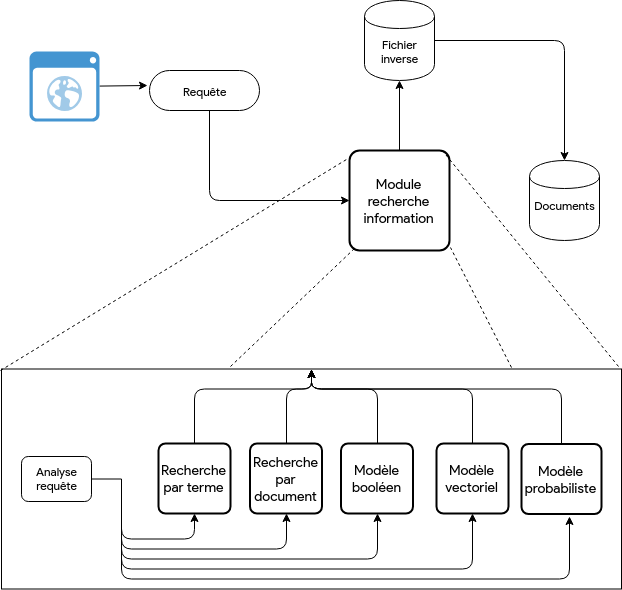
\includegraphics[width=0.65\linewidth]{images/systemdiag.png}
	\end{figure}
	\paragraph{}
	Il s'agit maintenant de décrire les différents composants du système, nous commencerons par
	la construction de l'indexe(fichier inverse) à partir des documents, puis l'analyse de la
	requête, enfin nous verrons l'implémentation de chaque modèle.
	
	\section{Construction de l'indexe}
	\paragraph{}
	La construction de l'indexe est très simple, nous faisons un parcours linéaire sur tout
	les documents pour construire la table d'indexation \textbf{Dico[d,t]}, chaque entrée 
	est la fréquence d'apparition du terme dans le document s'il existe.
	\paragraph{}
	Le bout de code suivant montre cette partie : 
	\begin{figure}[H]
		\centering
		\cutpic{0.3cm}{10cm}{images/gen_index.png}
	\end{figure}
	
	\paragraph{}
	Nous aurons plus tard besoin de calculer le poids d'un terme dans un document, la fonction
	suivante permet cela : 
	\begin{figure}[H]
		\centering
		\cutpic{0.3cm}{10cm}{images/weight.png}
	\end{figure}
	
	\section{Analyse de la requête}
	\paragraph{}
	Nous avons tout et en tout 3 types de requêtes :
	\begin{itemize}
		\item \textbf{Requête de recherche par terme simple} : constituée d'un mot clé simple
		pour la recherche à travers les documents
		\item \textbf{Requête de recherche par document} :
		numéro du document, affiche les termes qui sont dans le document avec leurs poids
		\item \textbf{Requête de recherche par mot clés multiple} : permet de rechercher un 
		ensemble de mot clé dans un ensemble de documents(Modèle booléen,vectoriel et probabiliste)
		
	\end{itemize}
	
	
	\section{Implémentation et évaluation du modèle booléen}
	\paragraph{}
	La fonction de similarité définie dans le chapitre 1 a été implémenté comme le 
	montre la capture suivante : 
	\begin{figure}[H]
		\centering
		\cutpic{0.3cm}{10cm}{images/boolean.png}
	\end{figure}
	
	\section{Implémentation et évaluation du modèle vectoriel}
	
	\subsection{Score d'un document }:
	\paragraph{}
	Par raison de simplicité, nous avons utilisé des \textbf{comprehension lists} 
	pour mieux traduire l'aspect mathématique des formules d'origine, voici le 
	code implémentant le calcul de ces mesure : 
	\begin{figure}[H]
		\centering
		\cutpic{0.3cm}{10cm}{images/vect_doc_score.png}
		\caption{Score d'un document}
	\end{figure}
	
	\begin{figure}[H]
		\centering
		\cutpic{0.3cm}{10cm}{images/vect_metrics.png}
		\caption{Les quatres mesures de similarité}
	\end{figure}
	
	\section{Implémentation et évaluation du modèle probabiliste}
	\paragraph{}
	Le modèle probabiliste se résumant au calcul d'une seule mesure de similarité,
	le code suivant contient son implémentation : 
	
	\begin{figure}[H]
		\centering
		\cutpic{0.3cm}{10cm}{images/proba_score.png}
		\caption{Calcul probabilité}
	\end{figure}
	
	
\chapter{Présentation de l'application}
	\section{Schéma d'utilisation}
	\paragraph{}
	Nous passon maintenant à la présentation de notre application pour l'exploitation
	des différents modules du système, l'application est divisée en 5 onglets, qui 
	contiennent chacun une interface dédié à l'approche qui lui est dédiée, voici une 
	capture d'écran annotée pour plus de clarté : 
	\begin{figure}[H]
		\centering
		\cutpic{0.1cm}{10cm}{images/app_screens/general.png}
		\caption{Interface génerale}
	\end{figure}
	
	\section{Exemples d'utilisation}
	\subsection{Recherche dans document}
	\paragraph{}
	Il suffit de donner le numero(nom) du document dans le champ dédié et de lancer 
	la recherche, le résultat est une liste de termes avec leurs poids associés, la
	capture suivante montre un exemple : 
	
	\begin{figure}[H]
		\centering
		\cutpic{0.1cm}{10cm}{images/app_screens/doc.png}
		\caption{Recherche dans un document}
	\end{figure}
	
	
	\subsection{Recherche par modèle booléen}
	\paragraph{}
	De manière semblable ç la recherche par terme, on introduit ici la requête dans
	le champ approprié, le résultat affiche les documents où le terme se trouve : 
	\begin{figure}[H]
		\centering
		\cutpic{0.1cm}{10cm}{images/app_screens/bool.png}
		\caption{Recherche booléenne}
	\end{figure}
	
	
	\subsection{Recherche par modèle vectoriel}
	\paragraph{}
	De la même façon, nous introduisant la liste de termes à rechercher dans leur champs,
	puis nous choisissons la mesure de similarité désirée, le résultat indique les documents
	résultants avec leurs scores : \\
	
	\begin{figure}[H]
		\centering
		\cutpic{0.1cm}{10cm}{images/app_screens/vect_cos.png}
		\caption{Recherche booléenne avec similarité cosinus }
	\end{figure}
	\begin{figure}[H]
		\centering
		\cutpic{0.1cm}{10cm}{images/app_screens/vect_jaccard.png}
		\caption{Recherche booléenne avec similarité de Jaccard}
	\end{figure}
	
	
	\subsection{Recherche par modèle probabiliste}
	\paragraph{}
	De manière analogue, nous introduisons les termes à rechercher dans le champ de recherche,
	puis nous donnons la main à l'utilisateur de sélectionner les documents pertinents pour 
	influencer la prochaine recherche, comme le montrent les deux captures suivantes :(une avant
	et l'autre après sélections des documents jugés \textbf{pertinents}) : 
	\begin{figure}[H]
		\centering
		\cutpic{0.1cm}{10cm}{images/app_screens/proba_1.png}
		\caption{Recherche probabiliste avec similarité par cosinus avant sélections}
	\end{figure}
	\begin{figure}[H]
		\centering
		\cutpic{0.1cm}{10cm}{images/app_screens/proba_2.png}
		\caption{Recherche probabiliste avec similarité par cosinus après sélections}
	\end{figure}
	
\chapter{Conclusion générale}
	\section{Analyse et comparaison}
	\paragraph{}
	Aux termes de ce projet, nous avons pu donc analyser les différentes méthodes 
	proposées, les implémenter nous a permis de mieux les comprendre et de percevoir
	leurs limites respectives.
	\paragraph{}
	Tout d'abord l'ajout d'un méthode d'indexation par fichier inverse à grandement
	diminué la complexité d'accès aux documents de la collections ainsi qu'à leur
	contenu. À ça s'ajoute l'utilisation de \textbf{stop\_words} pour éliminer les
	termes qui n'ont pas une valeur informationnelle, et donc ne sont pas présent
	dans l'indexe, en conséquent , la vitesse et la précision (rappel)de la 
	recherche sont accrus.
	\paragraph{}
	Le cœur d'un \textbf{SRI} \footnote{\textbf{S}ystème \textbf{R}recherche d'\textbf{I}nformation}
	reste néanmoins le modèle choisi pour le traitement d'une requête, de ce fait
	la performance du système dépend du choix de ce dernier, après l'implémentation
	des modèles, nous avons comparé leur performances (principalement la précision
	et le rappel et la rapidité d'exécution) :
	\paragraph{}
	Le modèle booléen, qui est le plus simple des trois, se veut être simple et
	intuitif, les principales forces de ce dernier sont sa facilité d'implémentation
	et sa grande rapidité d'exécution, en contre partie, la correspondance
	entre la requête et le document est très stricte, et ne diffère pas d'un 
	document pertinent à un autre, cela rend la tâche plus difficile à l'utilisateur
	quand il choisira quel document choisir. Pour palier à ce défaut le modèle 
	vectoriel à été introduit.
	\paragraph{}
	Le modèle vectoriel, un peu plus avancé que son prédécesseur, tente de discerner
	entre les documents pertinents, en introduisant la notion de similarité de
	document par rapport à une requête, ainsi même la formulation de cette dernière
	devient plus simple, et n'oblige pas l'utilisateur à avoir une idée précise de
	quels termes utiliser ou ne pas utiliser. Tout le challenge se trouve donc
	dans le choix de la mesure de similarité.
	
	\paragraph{}
	Une approche moins déterministe et plus probabiliste à vu le jour quand le 
	modèle probabiliste à été conçu, ce modèle se base sur un interprétation 
	stochastique du processus du choix de documents pertinents, en effet dans le
	monde réel, à l'instant de la formulation de la requête, le besoin de l'utilisateur
	est incertain, cette incertitude se retrouve aussi dans la manière dont
	les informations sont représentées, ce qui à poussé au choix de la théorie 
	des probabilité comme base théorique de ce modèle, afin de mesurer cette 
	quantité d'incertitude. Le modèle dépend grandement de deux facteurs : 
	\begin{itemize}
		\item L'hypothèse d'indépendance entre les termes dans un même document(alors 
		que ce n'est pas toujours le cas).
		\item Le chois de l'échantillon d'apprentissage doit être très bien étudié, car
		ce dernier représentera le concept de pertinence d'un document à travers
		tout le modèle.
	\end{itemize}
	Malgré ses restrictions, le modèle probabiliste de base donne de très bon résultats
	en terme de rappel et précision, cela en fait donc un bon point de départ pour
	le développement d'autres modèles plus performants et moins restreints.
	
	\section{Conclusion}
	\paragraph{}
	La recherche d’information présente des modèles assez intéressants qui ont pour fonction
	de permettre à l'utilisateur d'accéder à des documents qui contribuent à combler son besoin
	d'information, exprimé sous forme de requête, qui motive sa recherche. Ainsi le système
	peut être vu par l’utilisateur comme un instrument de prédiction de la pertinence des
	documents d’un corpus par rapport à sa requête.
	\par 
	De ce fait, la RI est un pilier du domaine de l’intelligence artificielle. Il est donc
	nécessaire d’améliorer ses résultats en s’intéressant aux besoins non exprimés de
	l’utilisateur pour augmenter la pertinence utilisateur/ machine.
	
\bibliographystyle{ieeetr}
\bibliography{ref}
\end{document}}

